\section{Otimização}
\label{s.optimization}

\begin{frame}{Otimização}
	\begin{itemize}
		\justifying
		\item A palavra matemática, do latim \emph{mathematica}, refere-se ao \textbf{conhecimento} e é considerada uma base formal para a resolução de problemas;
		\\~\\
		\item Alguns \textbf{problemas não são triviais} e necessitam de um conjunto adicional de ferramentas, conhecidas por otimização ou programação matemática.
		\end{itemize}
\end{frame}

\begin{frame}
	\begin{figure}
		\centering
		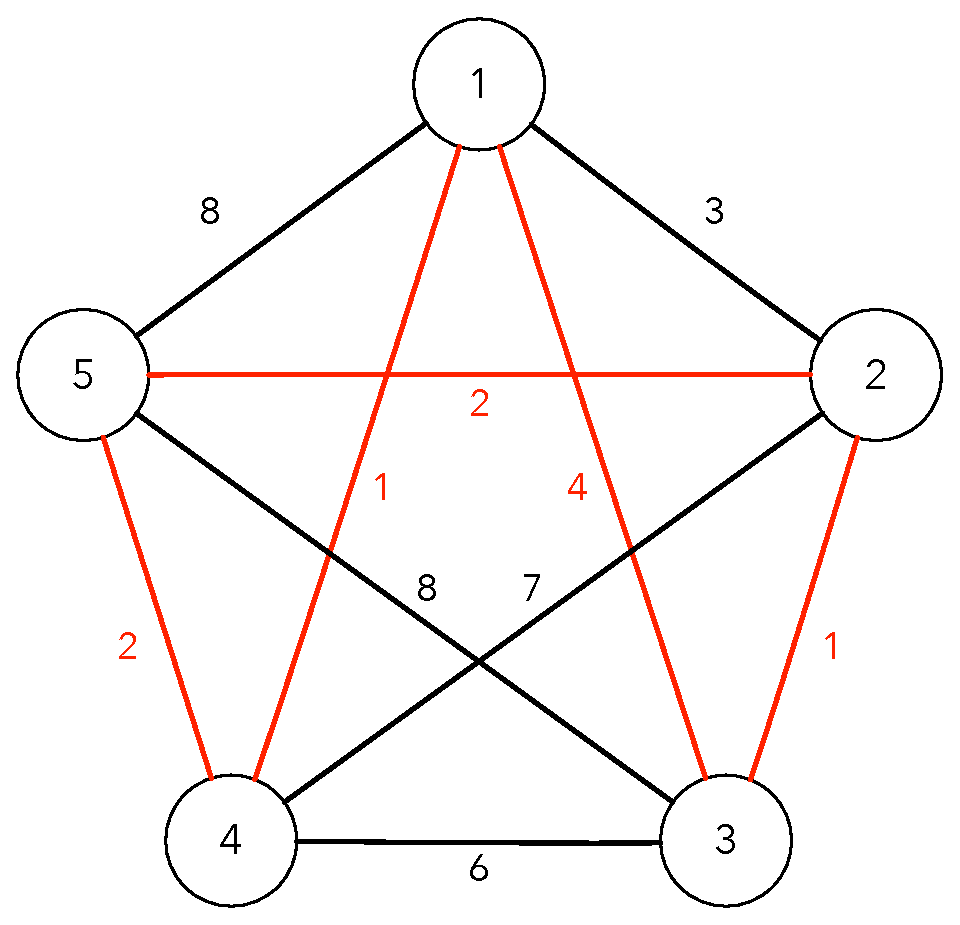
\includegraphics[scale=0.4]{figs/traveling_salesman.eps}	
		\caption{Ilustração do problema do Caixeiro Viajante~\cite{Papadimitriou:77}.}
		\label{f.traveling_salesman}
	\end{figure}
\end{frame}

\begin{frame}
	\textbf{Otimização} consiste em minimizar (maximizar) uma função matemática:
	\begin{equation}
		\label{e.min_opt}
		\min_{\forall \mathbf{x} \in {\Re^n}} f(\mathbf{x}),
	\end{equation}
	onde $f(\mathbf{x})$ é a função objetivo, dado que $\mathbf{x} \in \Re^n$. A otimização desta função objetivo visa encontrar o conjunto mais adequado de valores para $\mathbf{x}$, denominado por $\mathbf{x}^*$, onde $f(\mathbf{x}^*) \leq f(\mathbf{x})$.
	\\~\\
	\begin{block}{}
		\centering
			$\min(f) = \max(-f)$
	\end{block}	
\end{frame}

\begin{frame}
	\begin{figure}
		\centering
		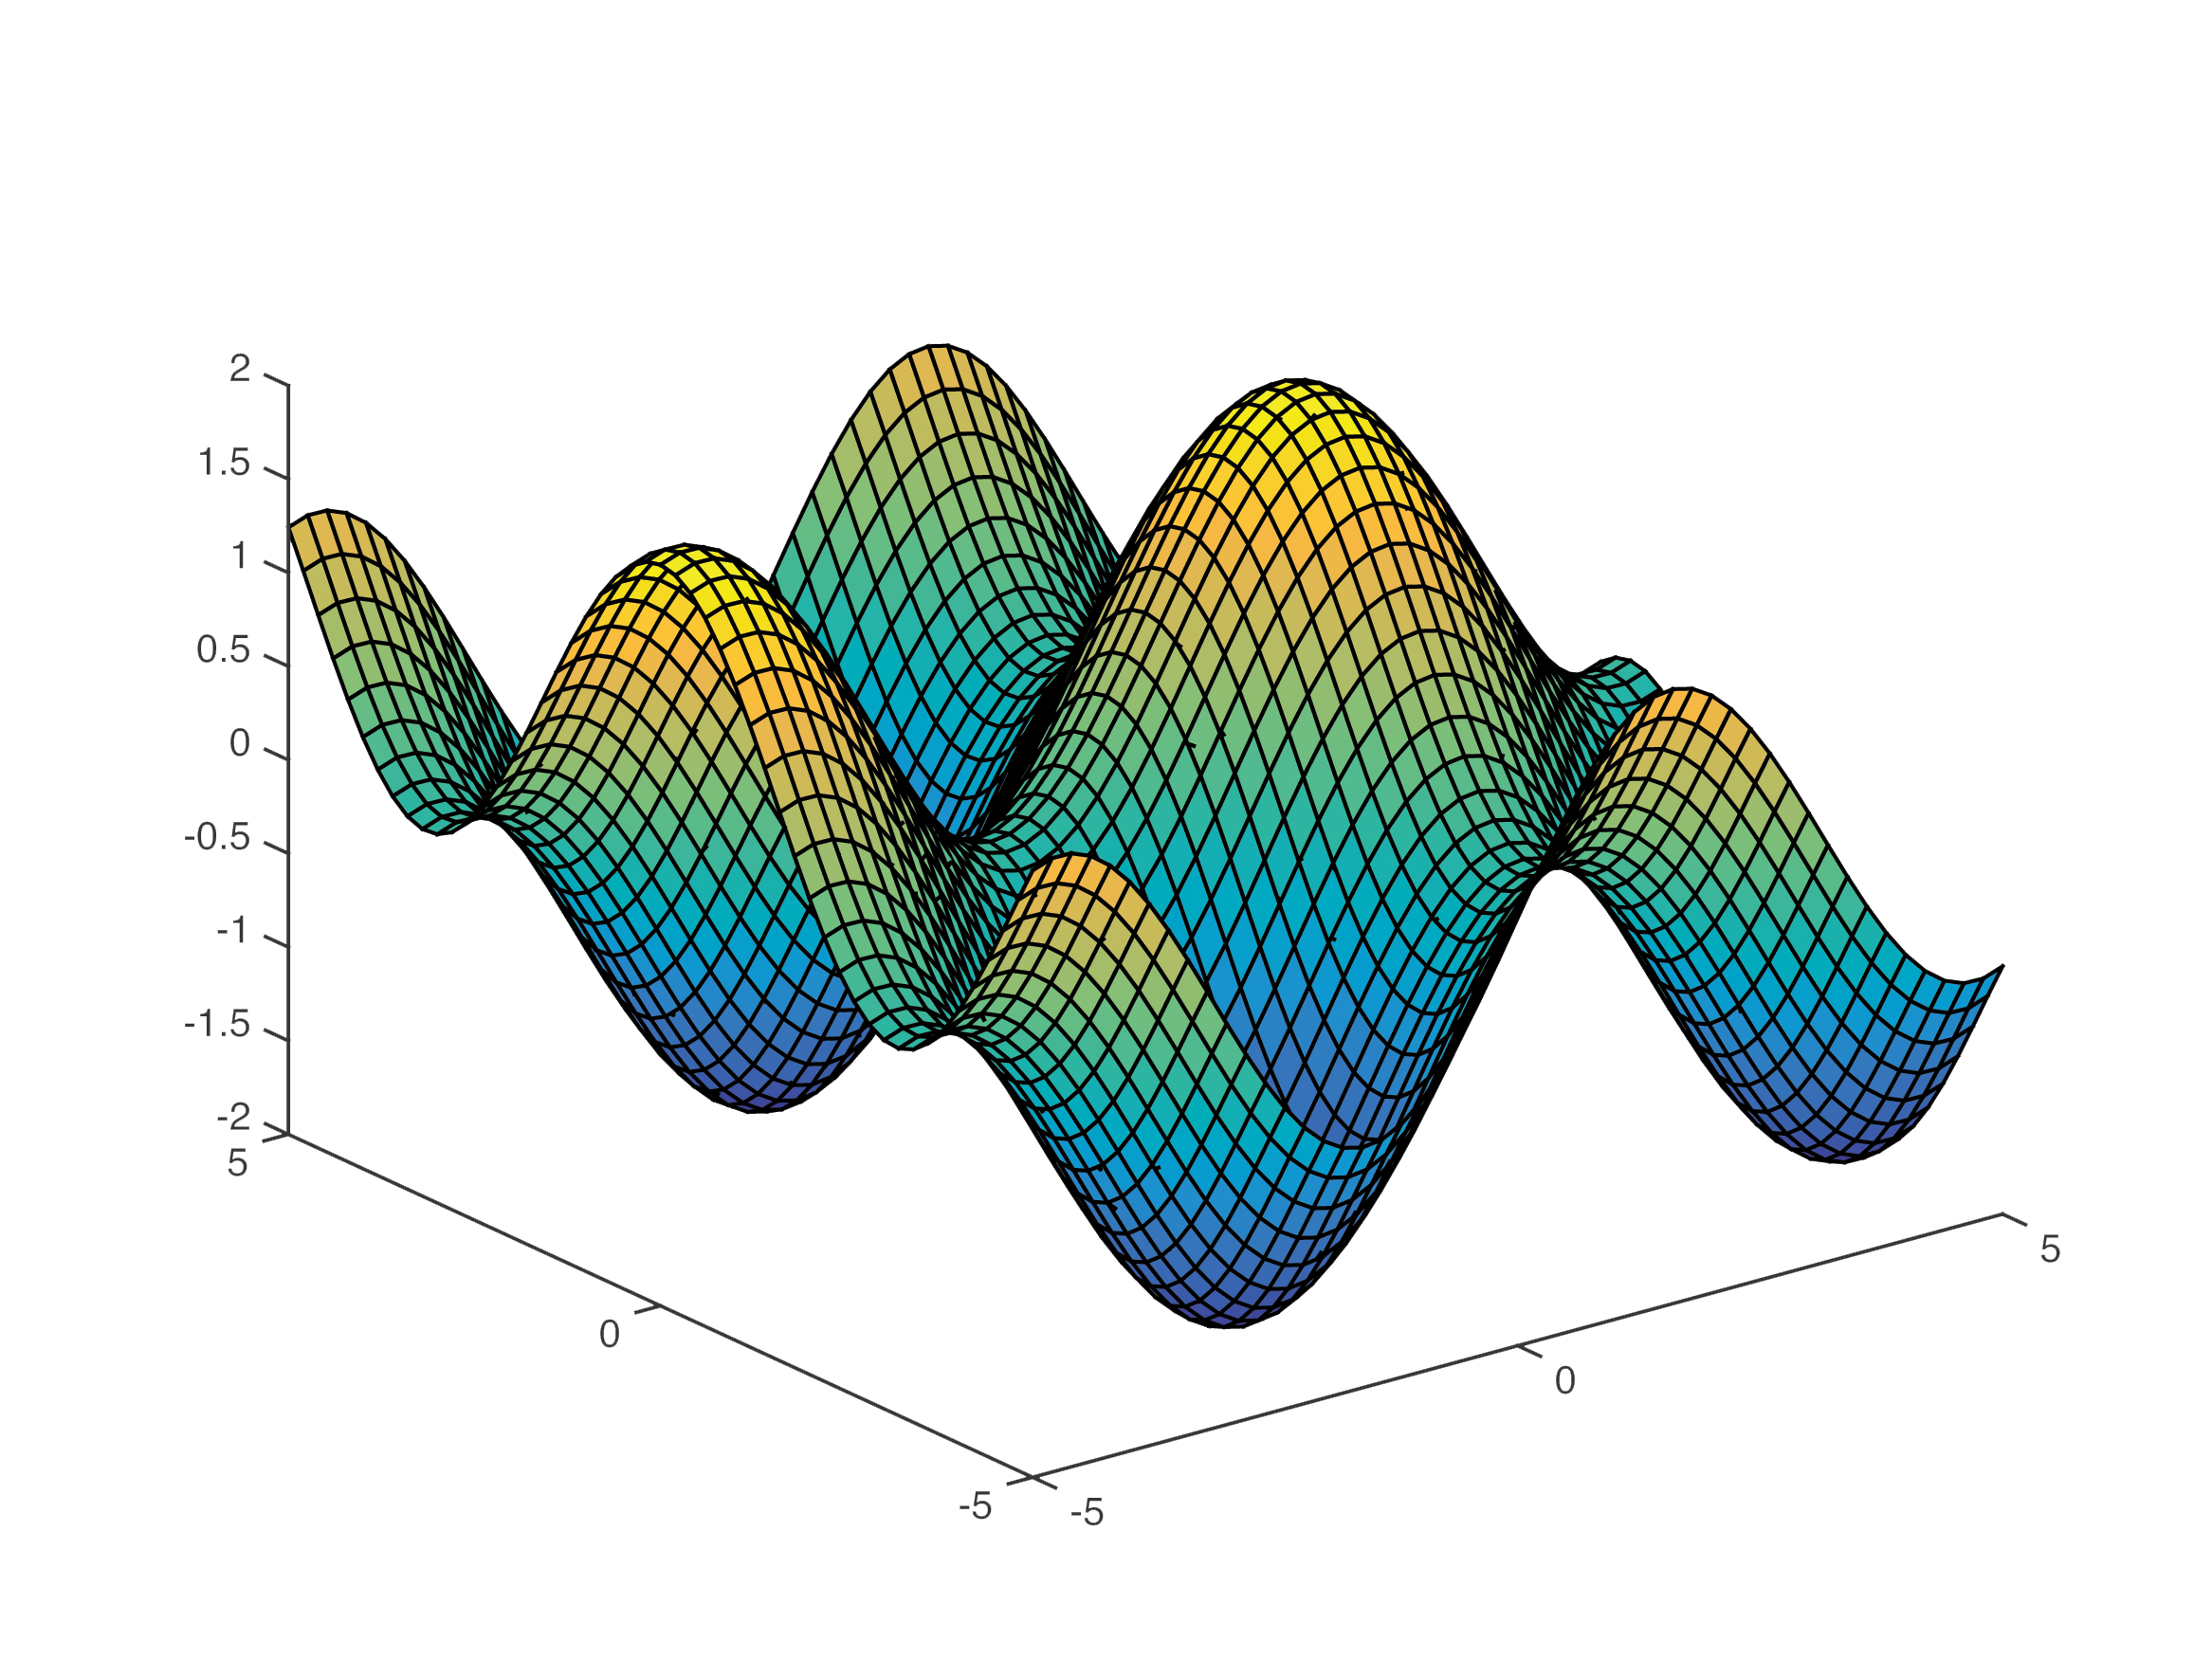
\includegraphics[scale=0.45]{figs/opt_function.png}	
		\caption{Exemplo de superfície da função $f(x,y)=sen(x)+cos(y)$.}
		\label{f.opt_function}
	\end{figure}
\end{frame}

\begin{frame}
	\begin{figure}
		\centering
		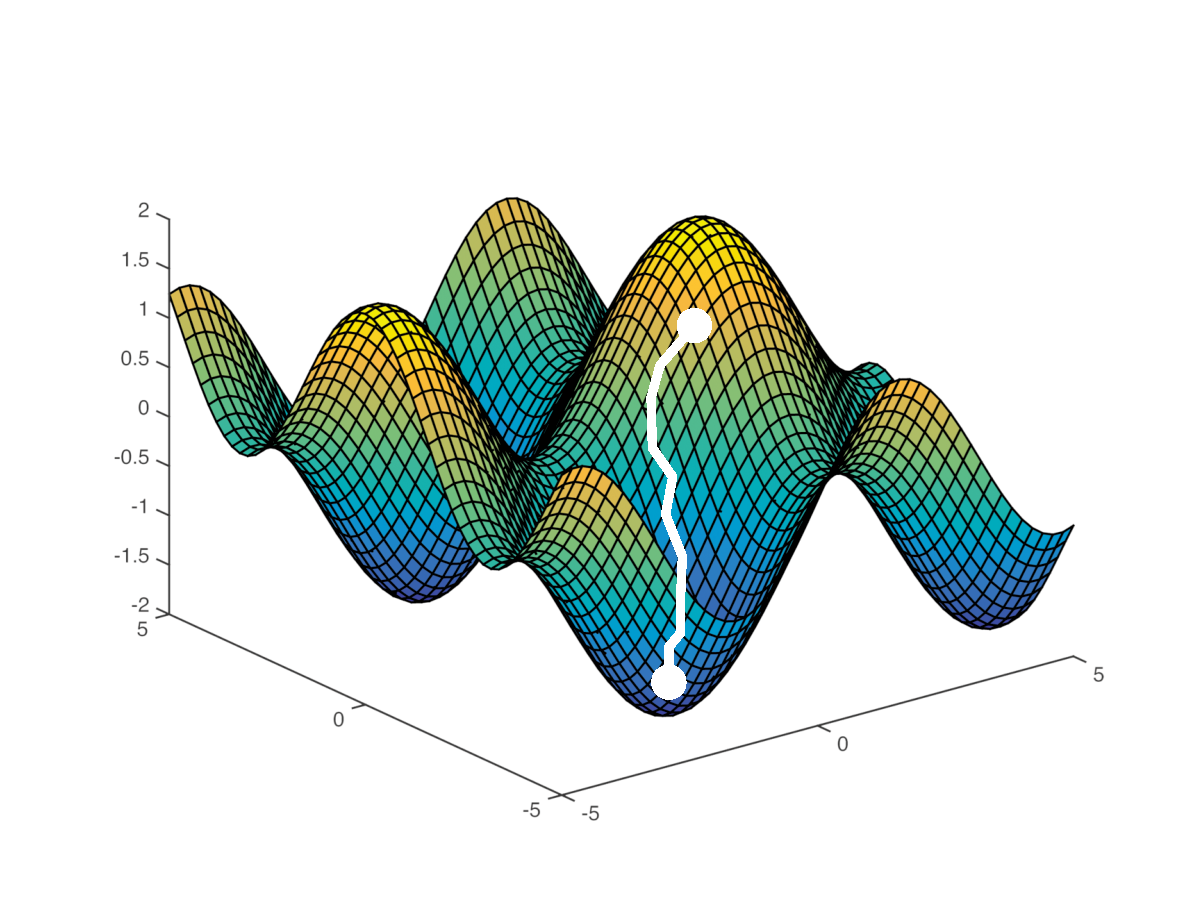
\includegraphics[scale=0.45]{figs/opt_function_opt.eps}	
		\caption{Exemplo de caminho realizado pelos passos da otimização até o encontro de um ponto de mínimo local.}
		\label{f.opt_function_opt}
	\end{figure}
\end{frame}

\begin{frame}
	\begin{itemize}
		\justifying
		\item Tradicionalmente, \textbf{métodos iterativos de otimização} são utilizados para a resolução de problemas de otimização;
		\\~\\
		\item Método de Newton, método Quasi-Newton, gradiente descendente, métodos de interpolação, dentre outros~\cite{Bertsekas:99};
		\\~\\
		\item Utilizam a \textbf{avaliação} de \textbf{gradientes}, Hessianos ou o próprio valor da função objetivo para encontrar as soluções ótimas.
	\end{itemize}
\end{frame}


\subsection{Otimização Meta-Heurística}
\label{ss.optimization_mh}

\begin{frame}{Otimização Meta-Heurística}
	\begin{itemize}
		\justifying
		\item Modelagem matemática de \textbf{fenômenos da natureza} em algoritmos de \textbf{otimização}~\cite{yang_review};
		\\~\\
		\item \textbf{Heurísticas} (buscas) de \textbf{soluções} em espaços $n$-dimensionais;
		\\~\\
	\end{itemize}
	\vspace*{0.5cm}
	\begin{block}{}
		\centering
		\textbf{Diversificação} x \textbf{Intensificação}
	\end{block}	
\end{frame}

\begin{frame}
	\begin{itemize}
		\justifying
		\item \textbf{Complexidade menor} quando comparadas aos métodos iterativos;
		\\~\\
		\item Simples \textbf{buscas locais} e procedimentos de aprendizado inspirados em comportamentos biológicos;
		\\~\\
		\item \textbf{Não} possuem \textbf{domínios específicos}.
	\end{itemize}
\end{frame}

\begin{frame}
	\begin{figure}
		\centering
		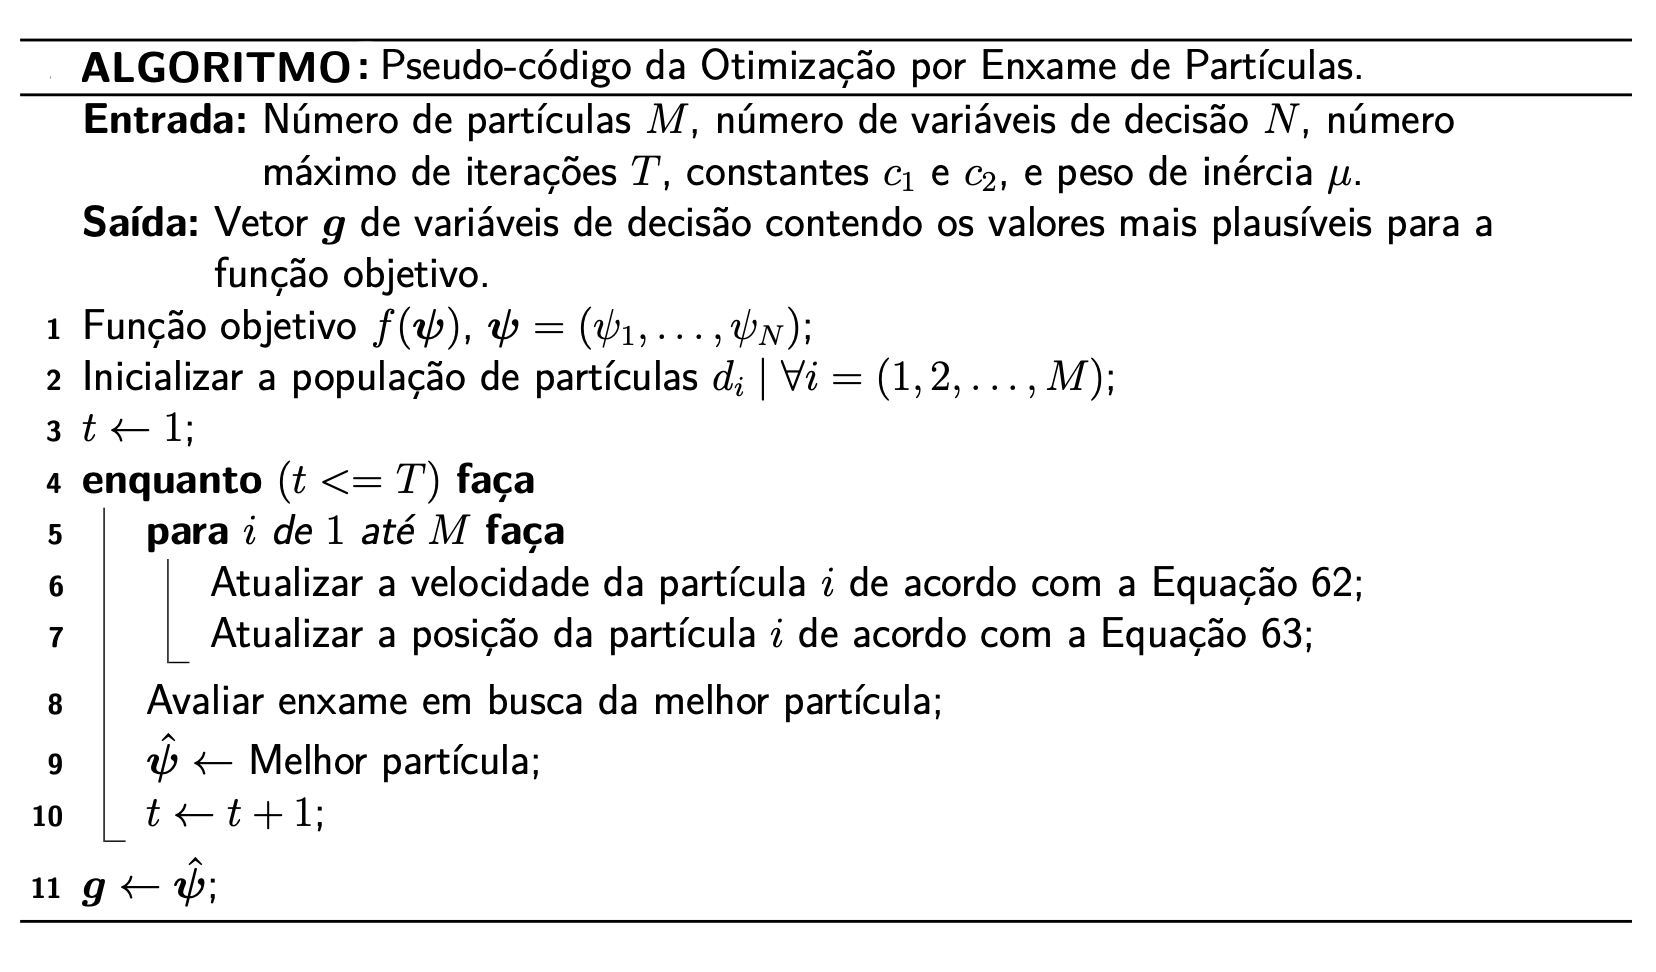
\includegraphics[scale=0.375]{figs/pso.png}	
		\caption{Pseudo-código da Otimização por Enxame de Partículas~\cite{Kennedy:01}.}
		\label{f.pso}
	\end{figure}
\end{frame}